\documentclass[a4paper,12pt]{article}
	\usepackage[left=2cm,right=1cm,top=1cm,bottom=1.5cm]{geometry}
	\usepackage[utf8]{inputenc}
	\usepackage[english,russian]{babel}
	\usepackage{graphicx}
	\usepackage{amsmath}
	\usepackage{amssymb}
	\usepackage{cite}
	\usepackage{indentfirst}
	\usepackage{multicol}
	\usepackage{cmap}
	
	\sloppy
	
	\usepackage{geometry}
	\geometry{top=2cm}
	\geometry{bottom=2cm}
	\geometry{left=2.5cm}
	\geometry{right=2.5cm}
	
	\renewcommand{\baselinestretch}{1.5}
	
	\begin{document}
		\renewcommand{\contentsname}{\Large Содержание}
		\renewcommand{\bibname}{\normalfont\Large\bfseries Список литературы}
		
		\begin{titlepage}
			\begin{center}
				Министерство науки и высшего образования Российской Федерации \\
				НАЦИОНАЛЬНЫЙ ИССЛЕДОВАТЕЛЬСКИЙ ЯДЕРНЫЙ УНИВЕРСИТЕТ <<МИФИ>> \\*
				\hrulefill
			\end{center}
		
		\begin{center}
			ИНСТИТУТ ЛАЗЕРНЫХ И ПЛАЗМЕННЫХ ТЕХНОЛОГИЙ\\
			КАФЕДРА №31 ПРИКЛАДНАЯ МАТЕМАТИКА
		\end{center}
		\vspace{1cm}
		
		\vspace{2em}
		
		\begin{center}
			\large{ОТЧЕТ}
			
			по научно-исследовательской работе
			за весенний семестр 2024 года \\
			
			на тему: Численное исследование уравнения Капицы
		\end{center}
		
		\begin{center}
			\large ТЕМА НИР
		\end{center}
	
	

\vspace{32em}
		
		\begin{center}
			г. Москва 2024
		\end{center}
	\end{titlepage}

	\newpage 
	\tableofcontents
	\setcounter{page}{3}
	
	\newpage
	\section*{Аннотация}
	
	В данной работе проводилось численное исследование уравнения Капицы, 
	включающее построение графиков зависимости фазы маятника Капицы от времени,
	и фазовых диаграмм. Также в работе была проведена проверка метода
	получения данных для графиков путем подбора задачи, похожей на исходную, 
	но с изветсным решением.
	
	\newpage
	\section{Введение}
	
	В данной работе рассматривается модель маятника Капицы, который
	представляет из себя комбинацию математического маятника и гармонического
	осцилятора (один из вариантов конструкции маятника представлен на 
	рисунке~\ref{fig:pend}).

	\begin{figure}[ht!]
		  \begin{center}
		  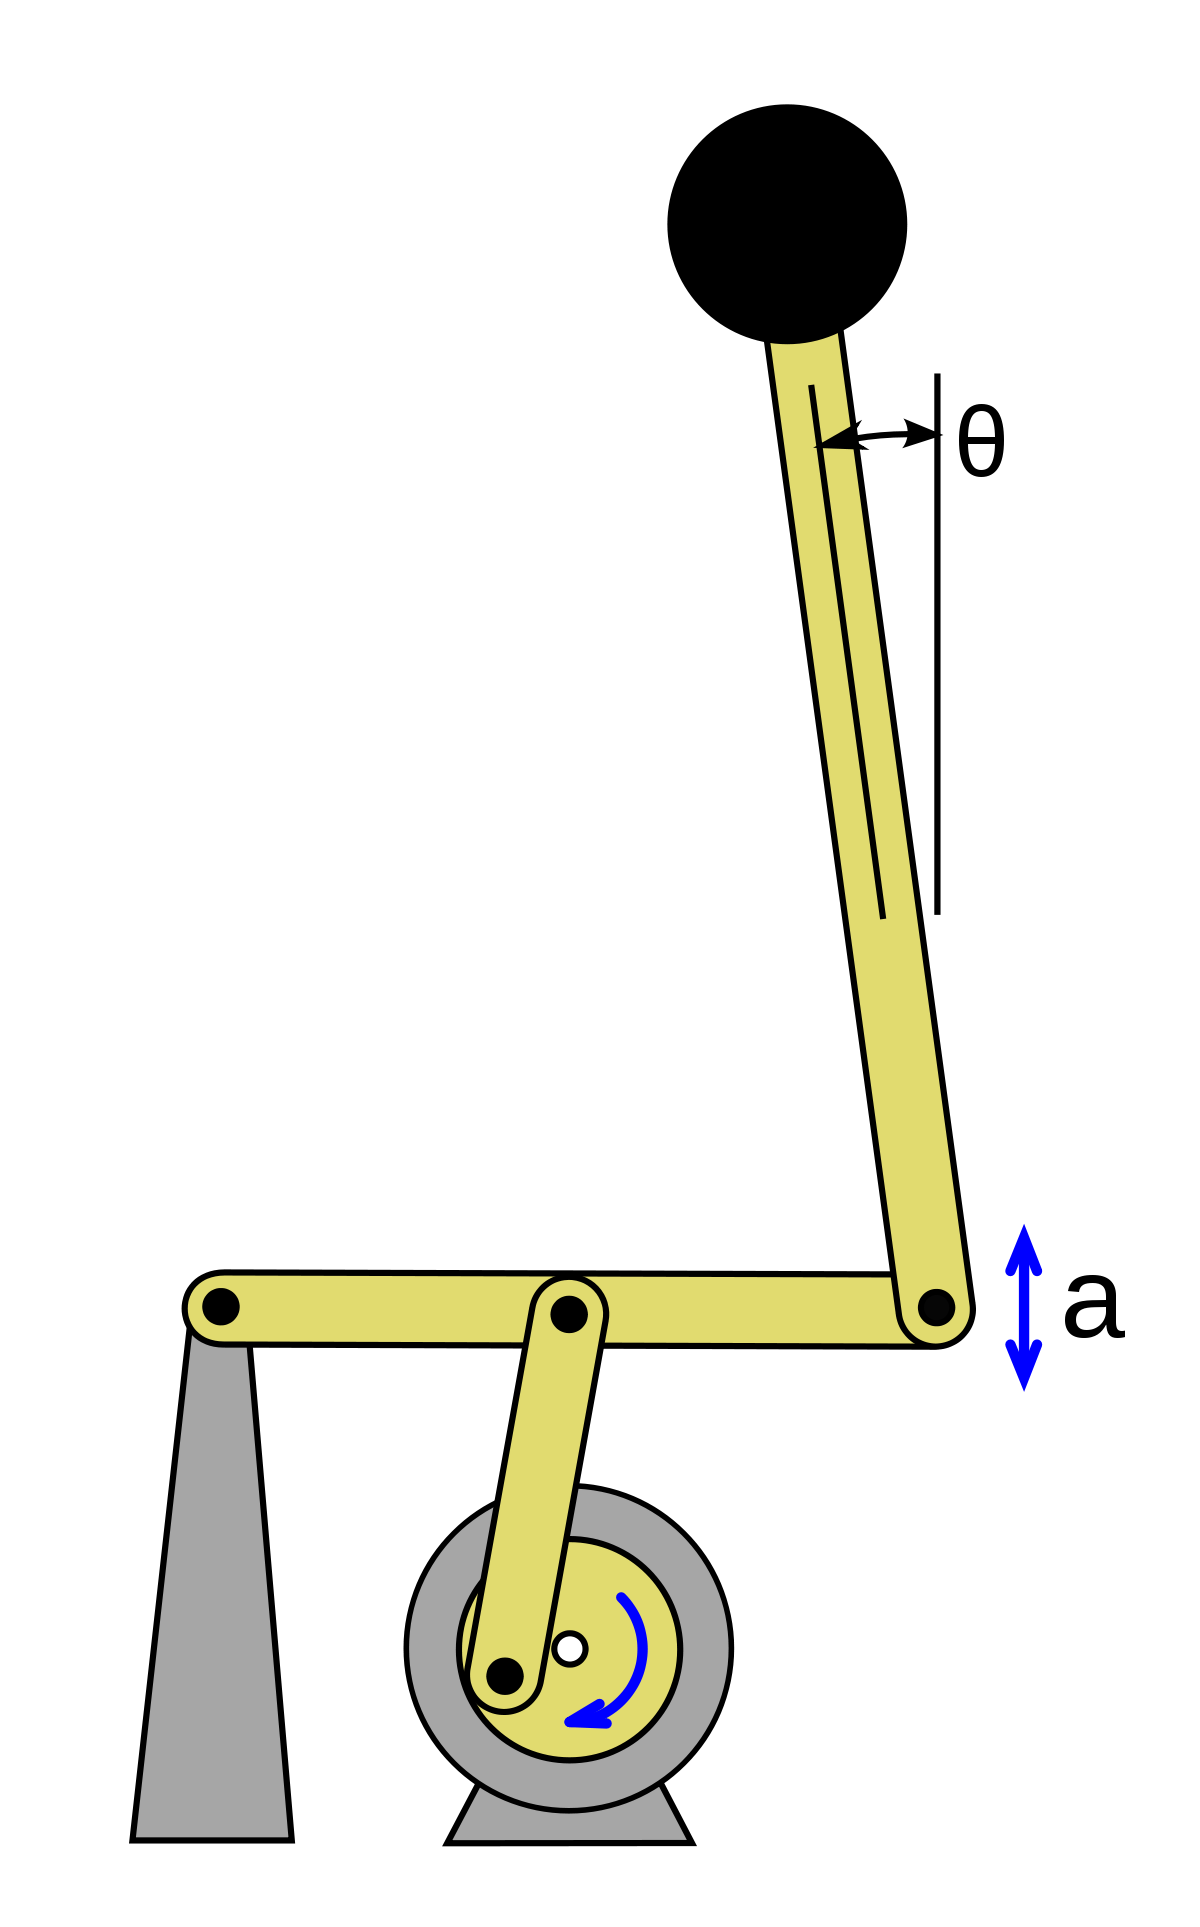
\includegraphics[scale=0.2]{sources/pend.png}
		  \end{center}
		  \vspace*{-8mm}
		  \caption{Пример конструкции маятника Капицы}\label{fig:pend}
	\end{figure}
	
	Данный маятник имеет два мехнизма, приводящие его в движение, что делает
	рисунок движения достаточно хаотичным. Существует дифференциальное 
	уравнение, описывающее движение данного маятника. Выглядит оно следующим
	образом:
	\begin{equation}L\phi^{\prime\prime} + (g - A\omega^2 \sin\omega t) \sin\phi = 0.\end{equation}

	В следующих разделах с целью исследования поведения маятника при разных
	условиях будет рассматриваться именно это уравнение.

	\newpage
	\section{Выбор метода интегрирования}
	Первым вопросом, который необходимо было решить,стал выбор метода 
	интегрирования. С помощью данного метода будут построены необходимые 
	графики, и получены необходимые данные о поведении функции при различных
	начальных условиях.

	Для проведения процесса интегрирования был выбран метод Рунге-Кутты 
	четвертого порядка. Это достаточно популярный метод решения подобных 
	задач. Четвертый порядок метода позволяет получить достаточно высокую
	точность измерения данных, чтобы проводить исследования при экстремальных 
	условиях работы установки, в нашем случае это высокая амплитуда, частота
	маятника. При этом данный порядок не достаточно высок, чтобы приводить 
	к существенному усложнению вычислений и запредельному времени работы 
	программы в целом. Также, как будет проверенно в дальнейшем, данный метод
	успешно справляется с тестовой задачей, и действительно показывает 
	четвертый порядок точности при ее решении.

	Суть данного метода заключается в вычислении каждой следующей фазы 
	положения через предыдущую. При этом в процессе происходит вычисление
	четырех вспомогательных коэффициентов.

	Рассмотрим задачу Коши для системы дифференциальных уравнений первого 
	порядка, и алгоритм получения значения $(x_{n+1}, t_{n+1})$ через 
	значение $(x_{n+1}, t_{n+1})$, где $x_n$ --- переменная, для которой
	происходит поиск значений, $t_n$ --- переменная, по которой произведено 
	дифференцирование. Задача Коши:
	\begin{equation}
		\begin{cases}
			x^\prime = f(x, t); \\
			x(t_0) = a.
		\end{cases}
	\end{equation}

	Первым шагом при переходе к новым значением становится вычисление 
	вспомогательных коэффициентов по следующим формулам:

	\newpage

	\begin{equation}
		k_1 = f(x_n, t_n)\tau,
	\end{equation}
	\begin{equation}
		k_2 = f(x_n + \frac12 k_1, t_n + \frac12 \tau)\tau,
	\end{equation}
	\begin{equation}
		k_3 = f(x_n + \frac12 k_2, t_n + \frac12 \tau)\tau,
	\end{equation}
	\begin{equation}
		k_4 = f(x_n + k_3, t_n + \tau)\tau.
	\end{equation}

	Далее происходит вычисление непосредственно самих новых значений 
	переменных. Для этого используется формула:

	\begin{equation}
		x_{n+1} = x_n + \frac16(k_1 + 2k_2 + 2k_3 + k_4)
	\end{equation}

	Таким образом получается рабочий метод Рунге-Кутты четвертого порядка, с
	помощью которого в дальнейшем будут полученны необходимые данные для 
	исследования уравнения Капицы и построения необходимых графиков.

	\section{Проверка метода с помощью тестовой задачи}

	Для того, чтобы убедиться в правильности выбора метода исследования
	данного уравнения, необходимо было проверить его на тестовой задаче, 
	которая была бы похожа на исходную, но при этом имела бы точное решение,
	позволяющее сравнить вычисленные значения с эталонными. Данной задачей 
	стало решение следующего уравнения (колебания гармонического маятника):
	\begin{equation}
		x^{\prime\prime} + \omega_0^2 x = 0.
	\end{equation}

	Данная задача имеет точное решение в виде:
	\begin{equation}
		x = A\cos(\omega_0t).
	\end{equation}
	
	В результате применения метода было полученно, что метод действительно 
	успешно справляется с поставленной задачей, а сравнение значений, 
	полученных с помощью численного интегрирования, с точными значениями, 
	полученными через точное решение действительно дало четвертый порядок 
	метода (см.~рисунок~\ref{fig:test}, на рисунке представлены необходимые
	графики самой задачи, логарифмической зависимости погрешности от шага
	измерений, в консоли можно увидеть результаты операции линейной регрессии
	логарифмической зависимости).

	\begin{figure}[ht!]
		  \begin{center}
		  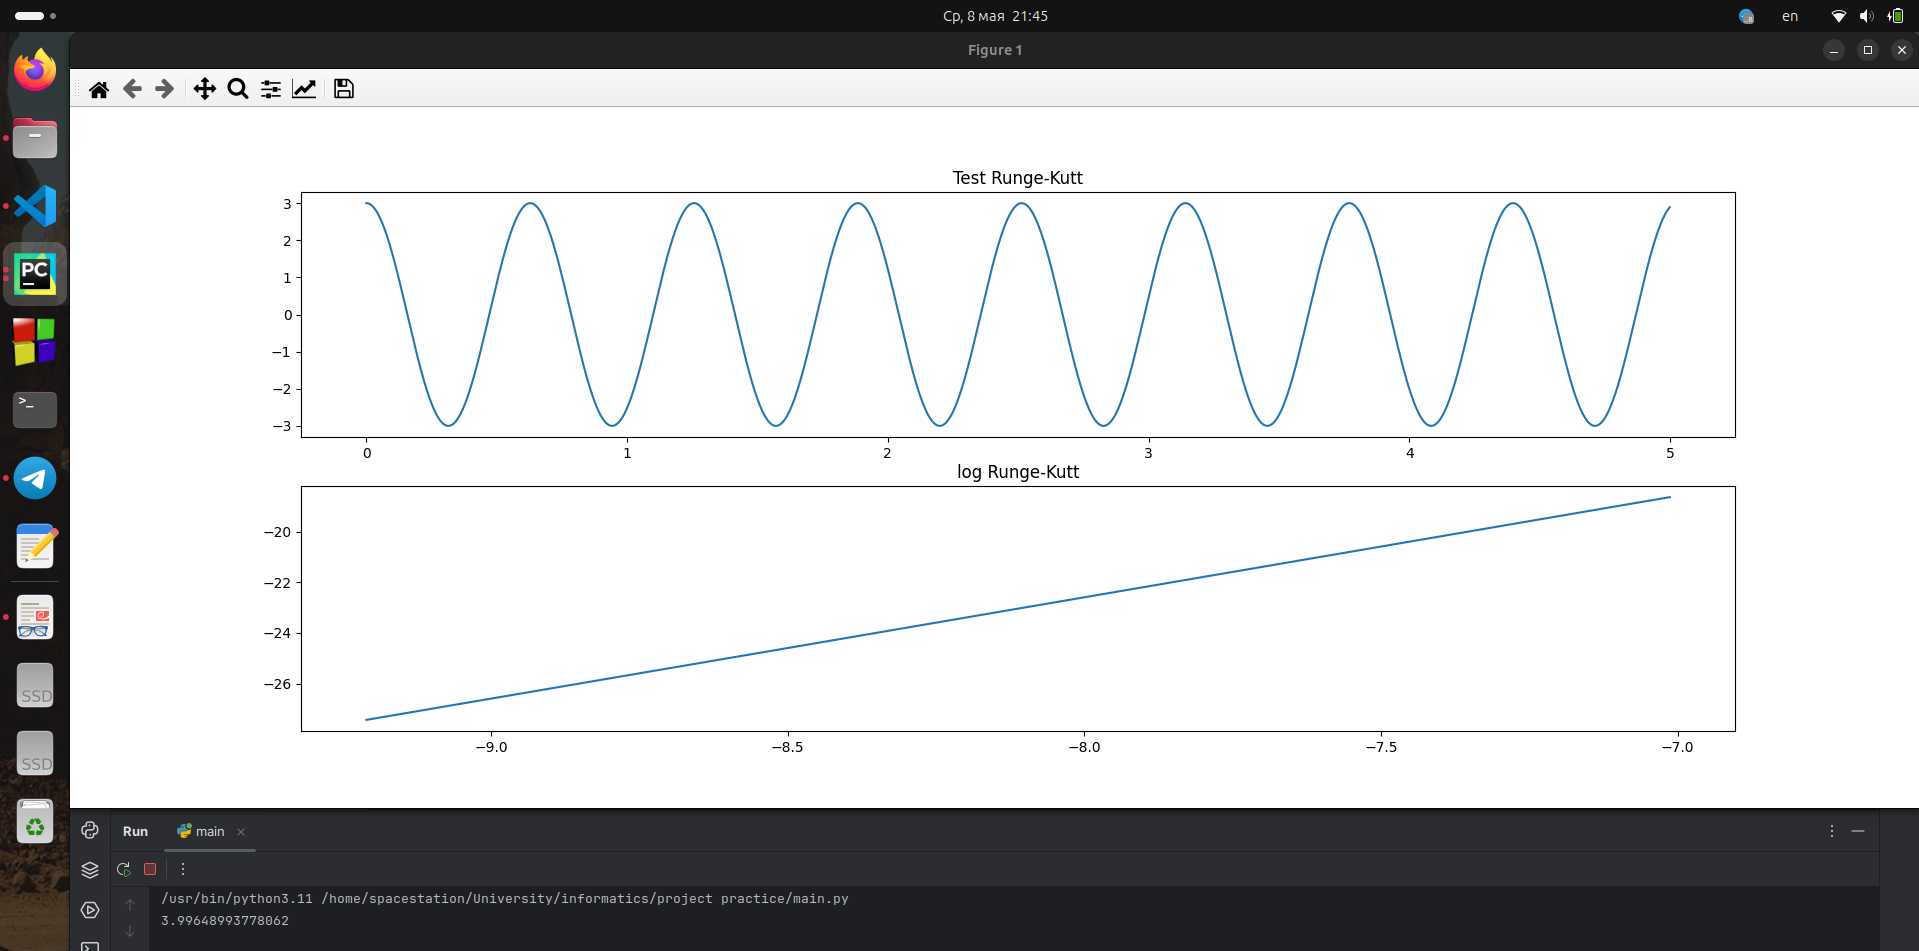
\includegraphics[scale=0.23]{sources/test.png}
		  \end{center}
		  \vspace*{-8mm}
		  \caption{Тестовая задача}\label{fig:test}
	\end{figure}

	\section{Интегрирование уравнения Капицы}
	На данном этапе работы было произведено вычисление необходимых 
	коэффициентов и подготовлена соответствующая программа для исследования 
	уравнения Капицы при различных начальных данных. В условии задачи было 
	предложено несколько наборов входных данных, для каждого из которых были 
	полученны соответствующие зависимости положения маятника от времени, а 
	также фазовые диаграммы. Они представлены ниже.
	\begin{enumerate}
		\item Условия (см.~рисунок~\ref{fig:1_praq}):
		\begin{equation}
			\begin{cases}
				A = 0.5; \\
				\omega = 5.3; \\
				\phi(0) = 3.1
			\end{cases}
		\end{equation}

		\newpage

		\begin{figure}[ht!]
			\begin{center}
			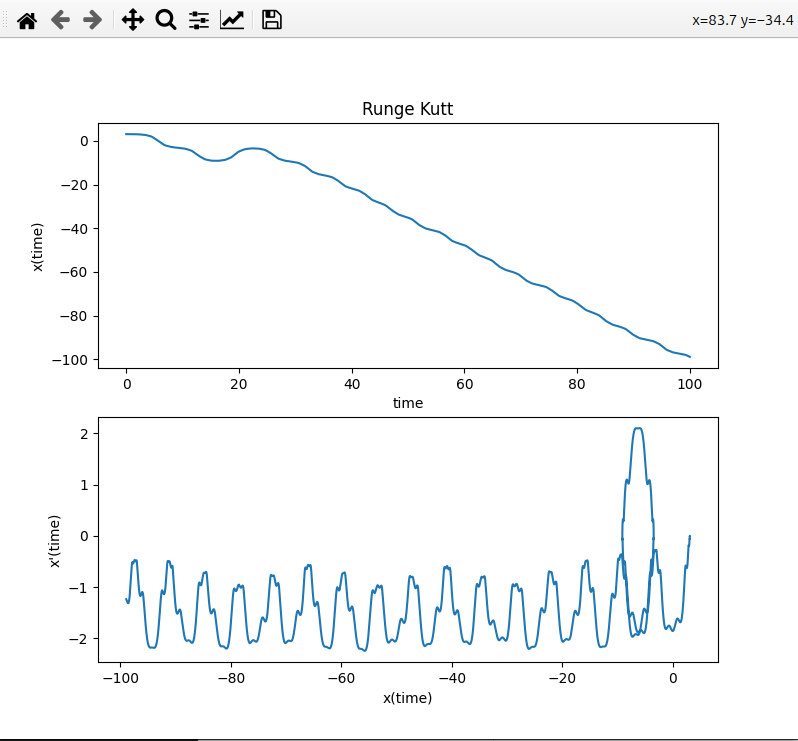
\includegraphics[scale=0.3]{sources/1_praq.png}
			\end{center}
			\vspace*{-8mm}
			\caption{Графики для первых условий}\label{fig:1_praq}
	  	\end{figure}

		\item Условия (см.~рисунок~\ref{fig:2_praq}):
		\begin{equation}
			\begin{cases}
				A = 10; \\
				\omega = 100; \\
				\phi(0) = 3.1
			\end{cases}
		\end{equation}
		\begin{figure}[ht!]
			\begin{center}
			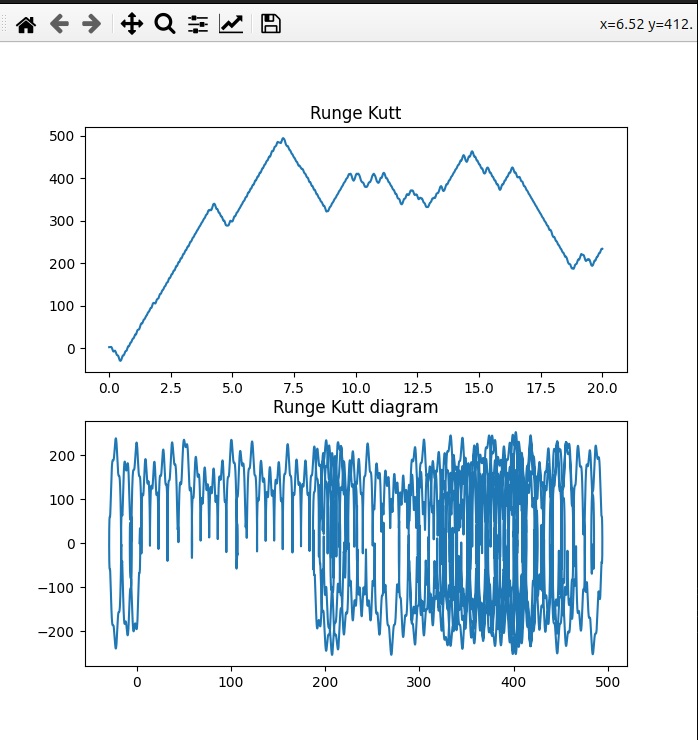
\includegraphics[scale=0.3]{sources/2_praq.png}
			\end{center}
			\vspace*{-8mm}
			\caption{Графики для вторых условий}\label{fig:2_praq}
	  	\end{figure}

		\item Условия (см.~рисунок~\ref{fig:3_praq}):
		\begin{equation}
			\begin{cases}
				A = 10; \\
				\omega = 100; \\
				\phi(0) = 0.1
			\end{cases}
		\end{equation}
		\begin{figure}[ht!]
			\begin{center}
			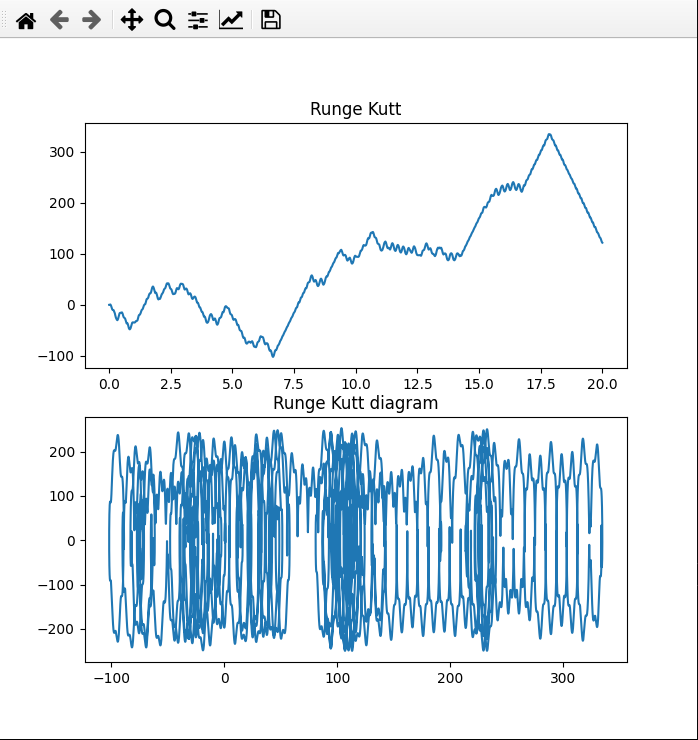
\includegraphics[scale=0.3]{sources/3_praq.png}
			\end{center}
			\vspace*{-8mm}
			\caption{Графики для третьих условий}\label{fig:3_praq}
	  	\end{figure}

		\item Условия (см.~рисунок~\ref{fig:4_praq}):
		\begin{equation}
			\begin{cases}
				A = 2; \\
				\omega = 100; \\
				\phi(0) = 0.1
			\end{cases}
		\end{equation}
		\begin{figure}[ht!]
			\begin{center}
			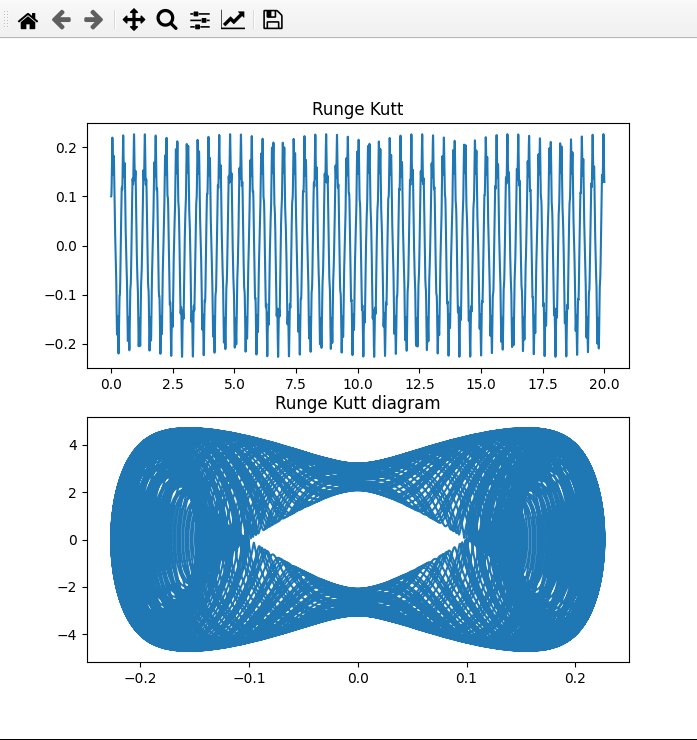
\includegraphics[scale=0.3]{sources/4_praq.png}
			\end{center}
			\vspace*{-8mm}
			\caption{Графики для четвертых условий}\label{fig:4_praq}
	  	\end{figure}

		\newpage

		\item Условия (см.~рисунок~\ref{fig:5_praq}):
		\begin{equation}
			\begin{cases}
				A = 0.5; \\
				\omega = 200; \\
				\phi(0) = 0.05
			\end{cases}
		\end{equation}
		\begin{figure}[ht!]
			\begin{center}
			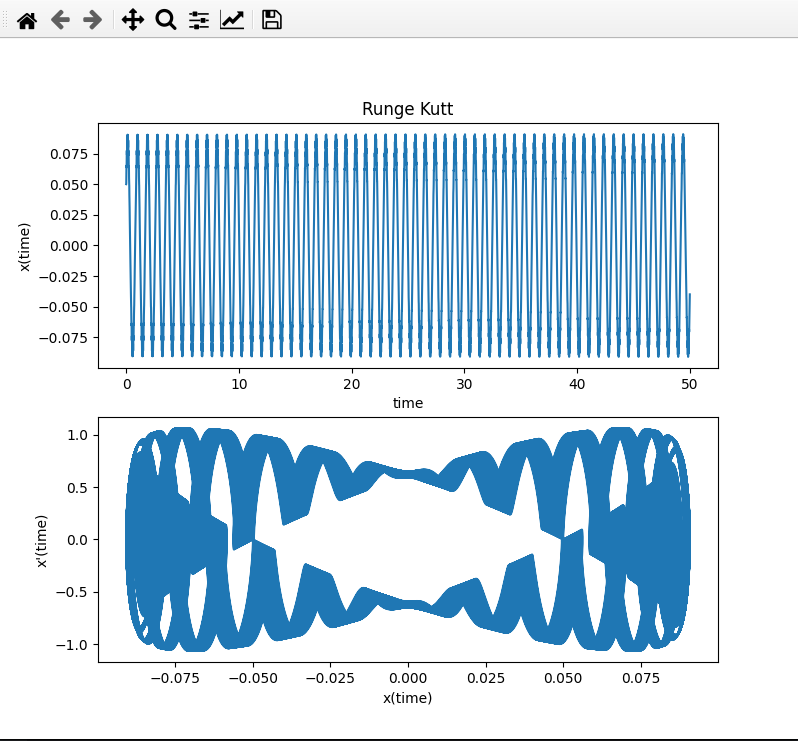
\includegraphics[scale=0.3]{sources/5_praq.png}
			\end{center}
			\vspace*{-8mm}
			\caption{Графики для пятых условий}\label{fig:5_praq}
	  	\end{figure}

	\end{enumerate}


	\newpage
	
	\section{Заключение}

	\begin{thebibliography}{w:40}
		
		\bibitem{label1} Боргояков Е. А., Кособрюхова О.В. "Современные подходы в профилактике неинфекционных заболеваний". - Ачинск. - 2016.
		
	\end{thebibliography}
	
	\end{document}